%%%%%%%%%%%%%%%%%%%%%%%%%%%%%%%%%%%%%%%%%%%%%%
% inspired from: https://tex.stackexchange.com/questions/580232/crisp-dm-diagram-with-tikz, correcting Deployment block and adjusting some styles

\documentclass[tikz,border=40pt]{standalone}

\usepackage{graphicx}
\usepackage{amsmath}
\usepackage{amsthm}
\usepackage{tikz}
\usetikzlibrary{chains, shapes.multipart}
\usetikzlibrary{shapes, calc, decorations.markings}
\usetikzlibrary{automata, positioning, fit, shapes.geometric}


\makeatletter
\tikzset{
    database/.style={
        path picture={
            \draw (0, 1.5*\database@segmentheight) circle [x radius=\database@radius,y radius=\database@aspectratio*\database@radius];
            \draw (-\database@radius, 0.5*\database@segmentheight) arc [start angle=180,end angle=360,x radius=\database@radius, y radius=\database@aspectratio*\database@radius];
            \draw (-\database@radius,-0.5*\database@segmentheight) arc [start angle=180,end angle=360,x radius=\database@radius, y radius=\database@aspectratio*\database@radius];
            \draw (-\database@radius,1.5*\database@segmentheight) -- ++(0,-3*\database@segmentheight) arc [start angle=180,end angle=360,x radius=\database@radius, y radius=\database@aspectratio*\database@radius] -- ++(0,3*\database@segmentheight);
        },
        minimum width=2.5*\database@radius + \pgflinewidth,
        minimum height=3*\database@segmentheight + 2*\database@aspectratio*\database@radius + \pgflinewidth,
    },
    database segment height/.store in=\database@segmentheight,
    database radius/.store in=\database@radius,
    database aspect ratio/.store in=\database@aspectratio,
    database segment height=0.1cm,
    database radius=0.5cm,
    database aspect ratio=0.5,
}
\makeatother


\begin{document}
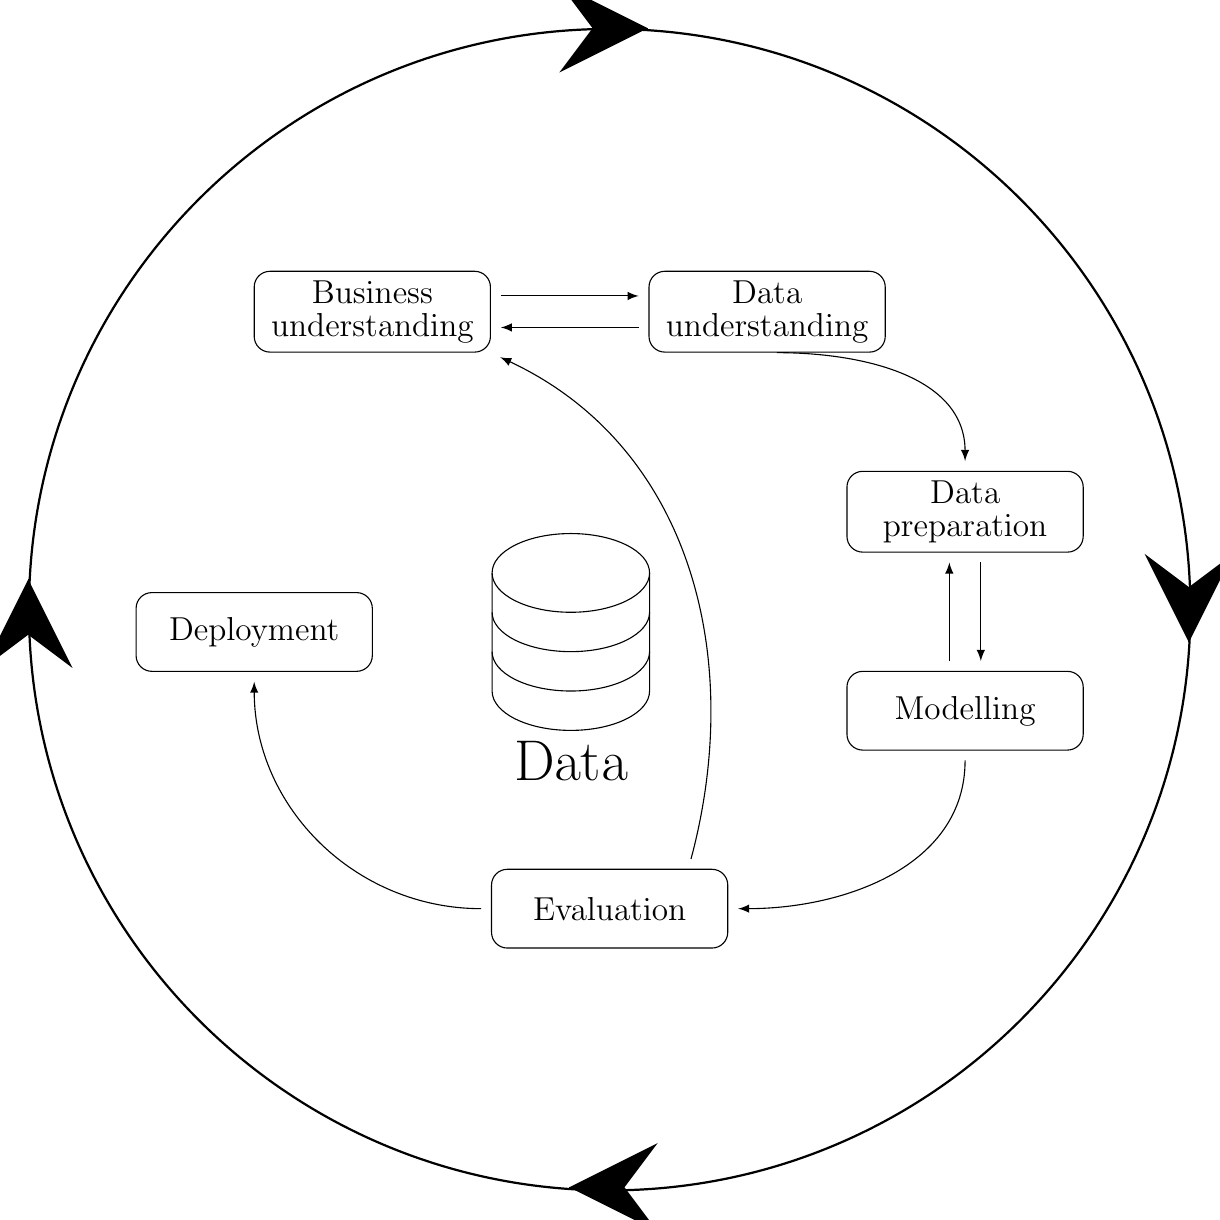
\begin{tikzpicture}[start chain=going right,>=latex,node distance=0pt]
    \node[draw, rectangle, align=center, rounded corners=2mm, minimum width=3cm, minimum height=1cm] (v1) {\large Business \\ \large understanding};
    \node[yshift=0.2cm] at (v1.east) (A1) {};
    \node[yshift=-0.2cm] at (v1.east) (A2) {};
    \node[draw, rectangle, align=center, rounded corners=2mm, minimum width=3cm, minimum height=1cm] (v2) [right=2cm of v1] {\large Data \\ \large understanding};
    \node[yshift=0.2cm] at (v2.west) (B1){};
    \node[yshift=-0.2cm] at (v2.west) (B2){};
    \node[draw, rectangle, align=center, rounded corners=2mm, minimum width=3cm, minimum height=1cm] (v3) [below right=1.5cm and -0.5cm of v2] {\large Data \\\large preparation};
    \node at (v2.south) (B3) {};
    \node at (v3.north) (C1) {};
    \node[draw, rectangle, align=center, rounded corners=2mm, minimum width=3cm, minimum height=1cm] (v4) [below=1.5cm of v3] {\large Modelling};
    \node[xshift=0.2cm] at (v3.south) (C2) {};
    \node[xshift=0.2cm] at (v4.north) (D1) {};
    \node[xshift=-0.2cm] at (v3.south) (C3) {};
    \node[xshift=-0.2cm] at (v4.north) (D2) {};
    \node[draw, rectangle, align=center, rounded corners=2mm, minimum width=3cm, minimum height=1cm] (v5) [below left=1.5cm and 1.5cm of v4] {\large Evaluation};
    \node at (v4.south) (D3) {};
    \node at (v5.east) (E1) {};
    \node[draw, rectangle, align=center, rounded corners=2mm, minimum width=3cm, minimum height=1cm] (v6) [above left=2.5cm and 1.5cm of v5] {\large Deployment};
    \node at (v5.west) (E2) {};
    \node at (v6.south) (F1) {};
    \node[database,label=below:\huge Data,database radius=1cm,database segment height=0.5cm] (v7) [right=1.25cm of v6] {};

    \draw [-latex] (A1) --+ (B1);
    \draw [-latex] (B2) --+ (A2);
    \draw [-latex] (B3) to [out=-0,in=90] (C1);
    \draw [-latex] (C2) --+ (D1);
    \draw [-latex] (D2) --+ (C3);
    \draw [-latex] (D3) to [out=-90,in=0] (E1);
    \draw [-latex] (E2) to [out=180,in=-90] (F1);
    
    \node[xshift=1.5cm] at (v1.south) (A3) {};
    \node[xshift=1cm] at (v5.north) (E3) {};
    \draw [-latex] (E3) to [out=75,in=-25] (A3);


    \draw [decoration={markings, mark=at position 1 with {\arrow[scale=10,>=stealth]{>}}}, postaction={decorate}] (3.4,3.6) -- (3.5,3.6);
    \draw [decoration={markings, mark=at position 1 with {\arrow[scale=10,>=stealth]{>}}}, postaction={decorate}] (2.6,-11.12) -- (2.5,-11.12);
    \draw [decoration={markings, mark=at position 1 with {\arrow[scale=10,>=stealth]{>}}}, postaction={decorate}] (10.37,-4.1) -- (10.37,-4.2);
    \draw [decoration={markings, mark=at position 1 with {\arrow[scale=10,>=stealth]{>}}}, postaction={decorate}] (-4.37,-3.5) -- (-4.37,-3.4);

    \node[circle, draw=black, decoration = {
        markings, 
        mark = at position 0.0  with {\arrow{latex}},
        mark = at position 0.25 with {\arrow{latex}}, 
        mark = at position 0.5  with {\arrow{latex}},
        mark = at position 0.75 with {\arrow{latex}},
    }, postaction = decorate,  thick, fit=(v1) (v2) (v3) (v4) (v5) (v6), inner sep=0pt] {};

\end{tikzpicture}
\end{document}